\section{多目的CAFE問題}\label{sec:background}

%-------------------------------------------------------
\begin{figure*}[t]\centering
  \begin{minipage}[b]{0.5\linewidth}
    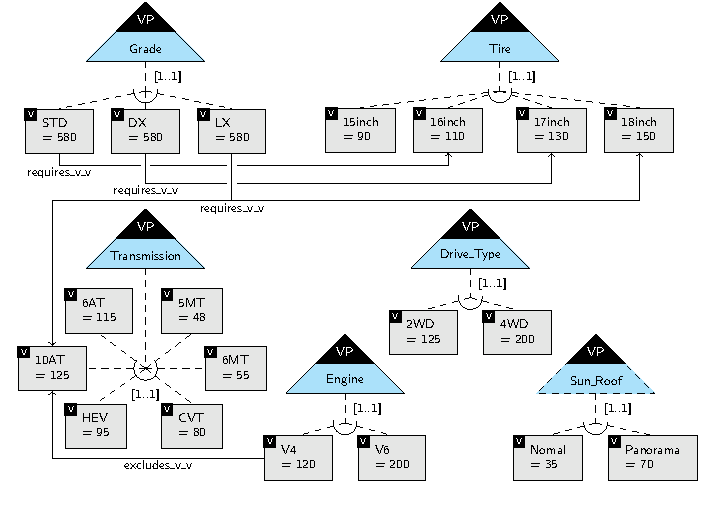
\includegraphics[width=1.0\linewidth]{images/ovm_example.pdf}
    \caption{CAFE問題の例}\label{fig:ovm}
  \end{minipage}\hfill
  \begin{minipage}[b]{0.4\linewidth}
    \begin{tabular}{l|c|c|c}\hline\hline
      & 車種1  & 車種2  & 車種3\\\hline
      \textsf{Grade}        & \textsf{STD}    & \textsf{DX}     & \textsf{LX}\\
      \textsf{Drive\_Type}  & \textsf{2WD}    & \textsf{2WD}    & \textsf{4WD}\\
      \textsf{Engine}	    & \textsf{V6}     & \textsf{V6}     & \textsf{V6}\\
      \textsf{Tire}	    & \textsf{16inch} & \textsf{17inch} & \textsf{18inch}\\
      \textsf{Transmission} & \textsf{6AT}    & \textsf{HEV}    & \textsf{10AT}\\
      \textsf{Sun\_Roof}    & -               & -               & -  \\\hline\hline
      IWR 値の総和           & 1,130  & 1,130   & 1,255 \\ %\hline
      燃費(km/L)      & 8.8  & 8.8     & 8.0 \\ %\hline
      予想販売台数    & 2,007   & 2,007   & 1,511  \\ \hline
      平均燃費(km/L)  & \multicolumn{3}{c}{8.5} \\ 
      予想販売台数(合計)  & \multicolumn{3}{c}{5,525} \\ 
      装備オプション数 & \multicolumn{3}{c}{12}	\\ \hline
    \end{tabular}
    \caption{CAFE 問題の解}\label{fig:ovm:ans}
\end{minipage}
\end{figure*}
%-------------------------------------------------------

図~\ref{fig:ovm}に CAFE 問題の例を示す.
この例は,ソフトウェアプロダクトライン開発の分野で用いられる
\textbf{可変性モデル} (Orthogonal Variability Model; OVM~\cite{Pohl05:sple})
によって記述されている.
%
\textsf{VP}でタグ付けされた三角形は,車種ごとに選択されるオプショ
ンが変わりうる\textbf{装備タイプ}を表す.
装備タイプの具体的な\textbf{装備オプション}は,
\textsf{V}でタグ付けされた長方形で表される.
長方形の中の数値は,IWR (Inertial Working Rating) と呼ばれ,
直観的には各装備オプションの重量を表す.
装備タイプと装備オプションの対応関係は,選択肢(破線)と
多重度($[lb..ub]$)で表される.
多重度の$lb$と$ub$は,それぞれ,各装備タイプで選択可能な装備オプション
数の上限値と下限値である.
装備タイプ同士,装備オプション同士,および,装備タイプと装備オプション
の間の依存関係は,実線矢印で表され,要求(\textsf{requires})と排他
(\textsf{excludes})の2種類がある.
%
図~\ref{fig:ovm}の問題例は,
6個のタイプ,19個のオプション,5個の依存関係から構成される.
各装備タイプの選択可能な装備オプション数はすべて1である.
例えば,
装備タイプ\textsf{Transmission}は,6つの装備オプション
\textsf{6AT},
\textsf{10AT},
\textsf{HEV},
\textsf{CVT},
\textsf{6MT},
\textsf{5MT}
からちょうど1つを選択可能である.また,
\textsf{10AT}と\textsf{V4}は,排他的な依存関係にある.
%
本論文では,
各車種に対して必須な装備タイプは実線のノードで表し,
\textsf{Sun\_Roof}のような必須でないものは破線のノードで表す.

車種数を$n$,
CAFE 基準値を$t$としたとき,
CAFE 問題の制約は以下の通りである.
\begin{description}
\item[範囲制約]: 各車種について,各装備タイプで選択される装備オプショ
    ン数は,与えられた上下限値の範囲内でなければならない.
\item[依存制約]: 各車種について,与えられた依存関係を満たさなければならない.
\item[燃費制約]: 車種$g\ (1\leq g\leq n)$の
  燃費と予想販売台数をそれぞれ$FE_{g}$と$SV_{g}$とするとき,
  以下の CAFE 規制を満たさなければならない.
\vskip -1em	  
  \[\begin{array}{lcr}
      & & \\
      \displaystyle\frac{\sum_{g=1}^{n} FE_{g}\cdot SV_{g}}{\sum_{g=1}^{n} SV_{g}}
      &
        \geq 
      &
        t \\
      & & 
   \end{array}\]
  不等式の左辺は,$n$車種の\textbf{平均燃費}を表している.
  $FE_{g}$と$SV_{g}$は,車種$g$におけるIWR値の総和から,
  企業が独自に保有する燃費テーブルと販売台数テーブルを基に計算される.
\end{description}

CAFE 問題の目的関数は,以下の通りである.
\begin{description}
 \item[予想販売台数の最大化]: 各車種ごとに求められる予想販売台数の合計を最大化する.
 \item[装備オプション数の最小化]: $n$車種全体で,使用される装備オプションの数を最小化する.
   これは,製造ラインの削減や,大量生産を促進することを狙いとしている.
\end{description}

本論文で対象とする多目的 CAFE 問題は,
与えられた問題インスタンス(可変性モデルで表現),
車種数$n$,
CAFE 基準値$t$,
燃費テーブルと販売台数テーブルから,
範囲制約,依存制約,燃費制約を満たしつつ,
予想販売台数の最大化と装備オプション数の最小化の2つの目的関数のもとで,
パレート最適解を求める問題である.

図~\ref{fig:ovm:ans}に,
問題インスタンス (図~\ref{fig:ovm}),
車種数$n=3$,
CAFE 基準値$t=8.5$に対する
実行可能解の一例を示す.
各車種の燃費は,左から順に 8.8, 8.8, 8.0km/L となり,
車種3は CAFE 基準値を満たしていないないが,
3台の平均燃費は 8.581km/L となり,CAFE 規制を満たしている.

%%% Local Variables:
%%% mode: latex
%%% TeX-master: "paper"
%%% End:
